\documentclass[12pt]{article}

\usepackage[margin=1.25in]{geometry}
\usepackage{fancyhdr}
\usepackage{setspace}
\renewcommand{\baselinestretch}{1.1}\pagestyle{fancy}
\pagestyle{fancy}
\usepackage{amsfonts}
\usepackage{listings}
\usepackage{amsthm}
\usepackage{amssymb,amsmath}
\usepackage{textpos}
\usepackage{enumerate}
\usepackage[utf8]{inputenc}
\usepackage[english]{babel}
\usepackage{mathtools}
\usepackage{verbatim}
\usepackage{graphicx}
\graphicspath{ {images/} }
\newcommand{\justif}[2]{&{#1}&\text{#2}}
\newcommand{\tx}[1]{\textnormal{#1}}
\newcommand{\bo}[1]{\boldsymbol{#1}}
\setlength{\parindent}{0pt}
\newcommand{\cc}[1]{#1)&}
\newcommand{\zz}[1]{\justif{\quad}{#1}\\}
\newcommand{\var}{\textnormal{var}}
\newcommand{\E}{\textnormal{E}}
\newcommand{\cov}{\textnormal{cov}}
\newcommand{\Poisson}{\textnormal{Poisson}}
\newcommand{\MSE}{\textnormal{MSE}}
\newcommand\independent{\protect\mathpalette{\protect\independenT}{\perp}}
\def\independenT#1#2{\mathrel{\rlap{$#1#2$}\mkern2mu{#1#2}}}
\usepackage{graphicx}

\lstset{
	language=R,
	basicstyle=\small\ttfamily,
	columns=flexible,
	breaklines=true,
	numbers=left
}

\title{Bikeshare}
\lhead{NonParametric Inference}
\chead{Bikeshare}
\rhead{Sam Baugh}

\begin{document}

Sam Baugh

NonParametric Inference \\

In a bike sharing system the process of obtaining membership, rental, and bike return is
automated via a network of kiosk locations throughout a city. In this problem, you will try
to combine historical usage patterns with weather data to forecast bike rental demand in the
Capital Bikeshare program in Washington, D.C.\\


You are provided hourly rental data collected from the Capital Bikeshare system spanning
two years. The file train.txt, as the training set, contains data for the first 19 days of
each month, while test.txt, as the test set, contains data from the 20th to the end of the
month. The dataset includes the following information:\\

\begin{itemize}
\item daylabel - day number ranging from 1 to 731 
\item year, month, day, hour - hourly date
\item season - 1 = spring, 2 = summer, 3 = fall, 4 = winter
\item holiday - whether the day is considered a holiday
\item workingday - whether the day is neither a weekend nor a holiday 
\item weather - 1 = clear, few clouds, partly cloudy 
\item 2 = mist + cloudy, mist + broken clouds, mist + few clouds, mist 
\item 3 = light snow, light rain + thunderstorm + scattered clouds, light rain + scattered clouds 
\item 4 = heavy rain + ice pallets + thunderstorm + mist, snow + fog 
\item temp - temperature in Celsius 
\item atemp - “feels like”  temperature in Celsius 
\item humidity - relative humidity
\item windspeed - wind speed
\item count - number of total rentals
\end{itemize}

Predictions are evaluated using the root mean squared logarithmic error (RMSLE), calculated
as $$\sqrt{\frac{1}{n}\sum_{n=1}^n(\log(m_i+1)-\log(\hat{m}_i+1))^2}$$

where $m_i$
is the true count, $\hat{m}_i$
is the estimate, and n is the number of entries to be evaluated.\\

\textbf{(a)} After various experimentation, we fit the following model. This was chosen as it has a relatively high $r^2$ and all of the factors are significant. The interaction terms generally make sense, as people's attitudes towards the weather may be different on a workday than a non-workday, and people might be more sensitive to temperature the second year. \\ 

NOTE: In this model the data was processed to factor holiday, workingday, season, and hour variables.

\begin{verbatim}
Call:
lm(formula = count ~ (month + factor(workingday) + temp + humidity + 
year + factor(hour)) + temp:year + month:humidity + workingday:temp + 
workingday:humidity + workingday:hour, data = hdata)
...
Adjusted R-squared:  0.9224 
\end{verbatim}

The RMSLE as computed on the validate set is $0.3919785$.\\

\textbf{(b)}

Below is the scattered plot of average hourly logged count against daylabel. We can see a strong trend through time.

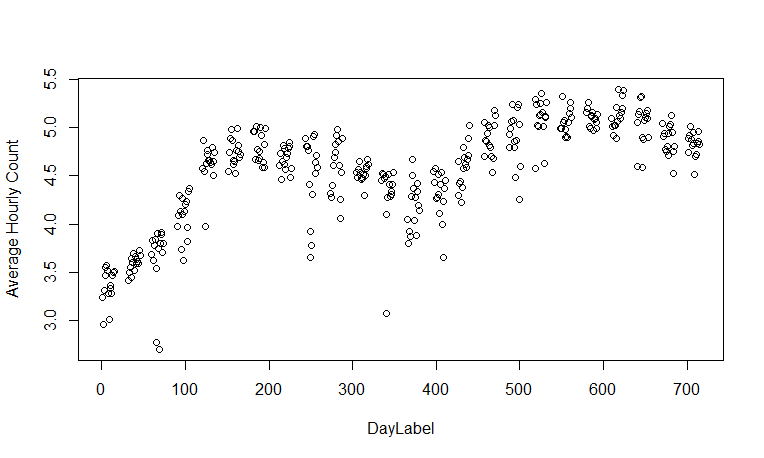
\includegraphics[scale=0.5]{daylabel_avg}

The graph below shows our plot of risk versus bandwidth using the tricube kernel. We see that $h\approx 40$ is the optimal bandwidth.

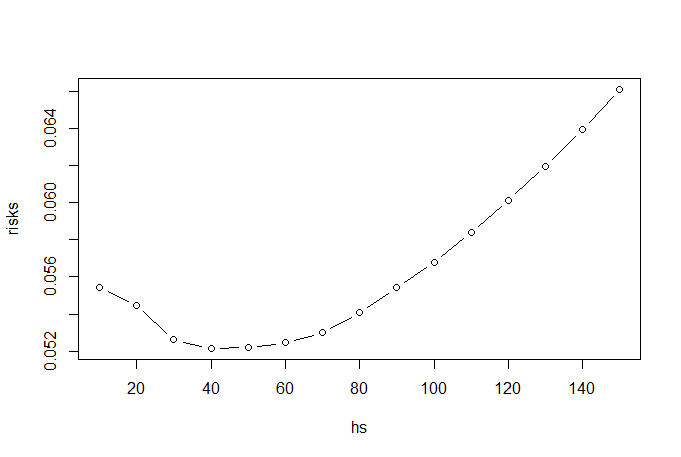
\includegraphics[scale=0.5]{risks}

The following graph shows our fit of the kernel smoother with the optimal bandwidth, using the tricube kernel.

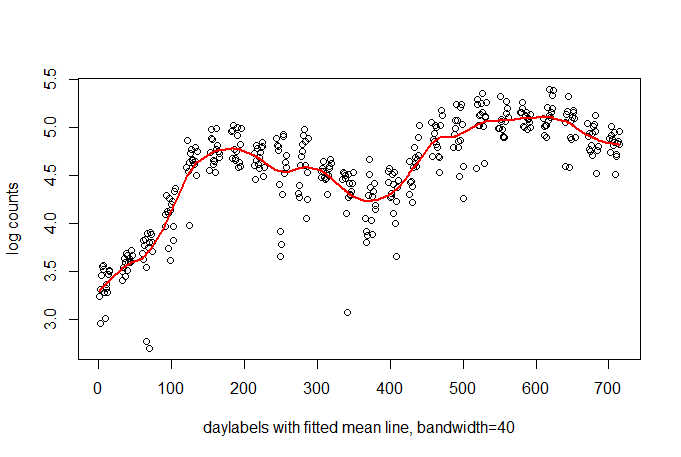
\includegraphics[scale=0.5]{fitt}



We then de-trend the hourly data, fit the model from part (a) to the residuals, predict the residuals on the validate set, and then re-trend the validate set to get a new set of predictions. We get an RMSLE of $1.018996$.\\

\textbf{(c)} After some experimentation with the data, we fit the general additive model

\begin{verbatim}
Call: gam(formula = count ~ (daylabel + temp + factor(hour) + humidity + 
year) + daylabel:humidity + daylabel:temp + daylabel:humidity + 
hour:humidity + humidity:year, data = hdata)
Deviance Residuals:
Min       1Q   Median       3Q      Max 
-3.61615 -0.30620  0.03844  0.37600  2.35343 

(Dispersion Parameter for gaussian family taken to be 0.378)

Null Deviance: 18298.36 on 8639 degrees of freedom
Residual Deviance: 3245.305 on 8586 degrees of freedom
AIC: 16169.03 

Number of Local Scoring Iterations: 2 

Anova for Parametric Effects
Df  Sum Sq Mean Sq   F value    Pr(>F)    
daylabel             1  1187.5 1187.47 3141.6567 < 2.2e-16 ***
temp                 1  2151.6 2151.62 5692.4742 < 2.2e-16 ***
factor(hour)        23 11563.2  502.75 1330.1023 < 2.2e-16 ***
humidity             1    54.2   54.18  143.3539 < 2.2e-16 ***
year                 1    29.6   29.56   78.2102 < 2.2e-16 ***
daylabel:humidity    1    11.0   11.03   29.1687 6.812e-08 ***
daylabel:temp        1    35.8   35.80   94.7272 < 2.2e-16 ***
humidity:hour       23    17.6    0.77    2.0251  0.002585 ** 
humidity:year        1     2.6    2.59    6.8610  0.008825 ** 
Residuals         8586  3245.3    0.38                        
---
Signif. codes:  0 ‘***’ 0.001 ‘**’ 0.01 ‘*’ 0.05 ‘.’ 0.1 ‘ ’ 1
\end{verbatim}

We get a RMSLE of $0.5982461$ on the validate set. \\


\end{document}
